
\noindent\begin{minipage}{\textwidth}
    \begin{table}[H]
        \centering
        \caption{Hiperparâmetros e Resultados do Melhor Modelo - resnet\_v10\_BR\_opt\_aug}
        \vspace{0.2cm}
        \resizebox{\textwidth}{!}{%
            \begin{tabular}{ll | lrrr}
                \hline
                \multicolumn{2}{c|}{\textbf{Hiperparâmetros}} & \multicolumn{4}{c}{\textbf{Métricas por Classe}} \\ \hline
                \textbf{Parâmetro} & \textbf{Valor} & \textbf{Classe} & \textbf{Precisão} & \textbf{Recall} & \textbf{F1-Score} \\ \hline
    Agendador de LR & StepLR & 31.2 & 0,4069 & 0,8468 & 0,5497 \\ 
Architecture & resnet50 & 31.3 & 0,4667 & 0,2606 & 0,3345 \\ 
Augmentation (Método) & None & 31.4 & 0,4407 & 0,4561 & 0,4483 \\ 
Batch Size & 32 & 32.3 & 0,6205 & 0,6402 & 0,6302 \\ 
Decaimento de Peso (WD) & 0,0001 & 32.4 & 0,2500 & 0,5000 & 0,3333 \\ 
Dropout & 0,3002 & 33.3 & 0,7586 & 0,3056 & 0,4356 \\ 
Função de Perda & CrossEntropyLoss & 41.4 & 0,5909 & 0,2766 & 0,3768 \\ 
Hidden Units & 512 & 41.5 & 0,8333 & 0,4651 & 0,5970 \\ 
Label Smoothing & 0,1000 & 42.4 & 0,8000 & 0,3934 & 0,5275 \\ 
Otimizador & AdamW & 44.4 & 0,7931 & 0,7188 & 0,7541 \\ 
\cline{3-6} 
Taxa de Aprendizado (LR) & 1,76e-04 & \textbf{Média (Macro)} & 0,5951 & 0,5252 & 0,5362 \\ 
Unfreeze Layers & 3 & \textbf{MCC} & \multicolumn{3}{c}{0,4823} \\ 
            \hline
            \end{tabular}%
        }
    \end{table}

    \begin{figure}[H]
        \centering
        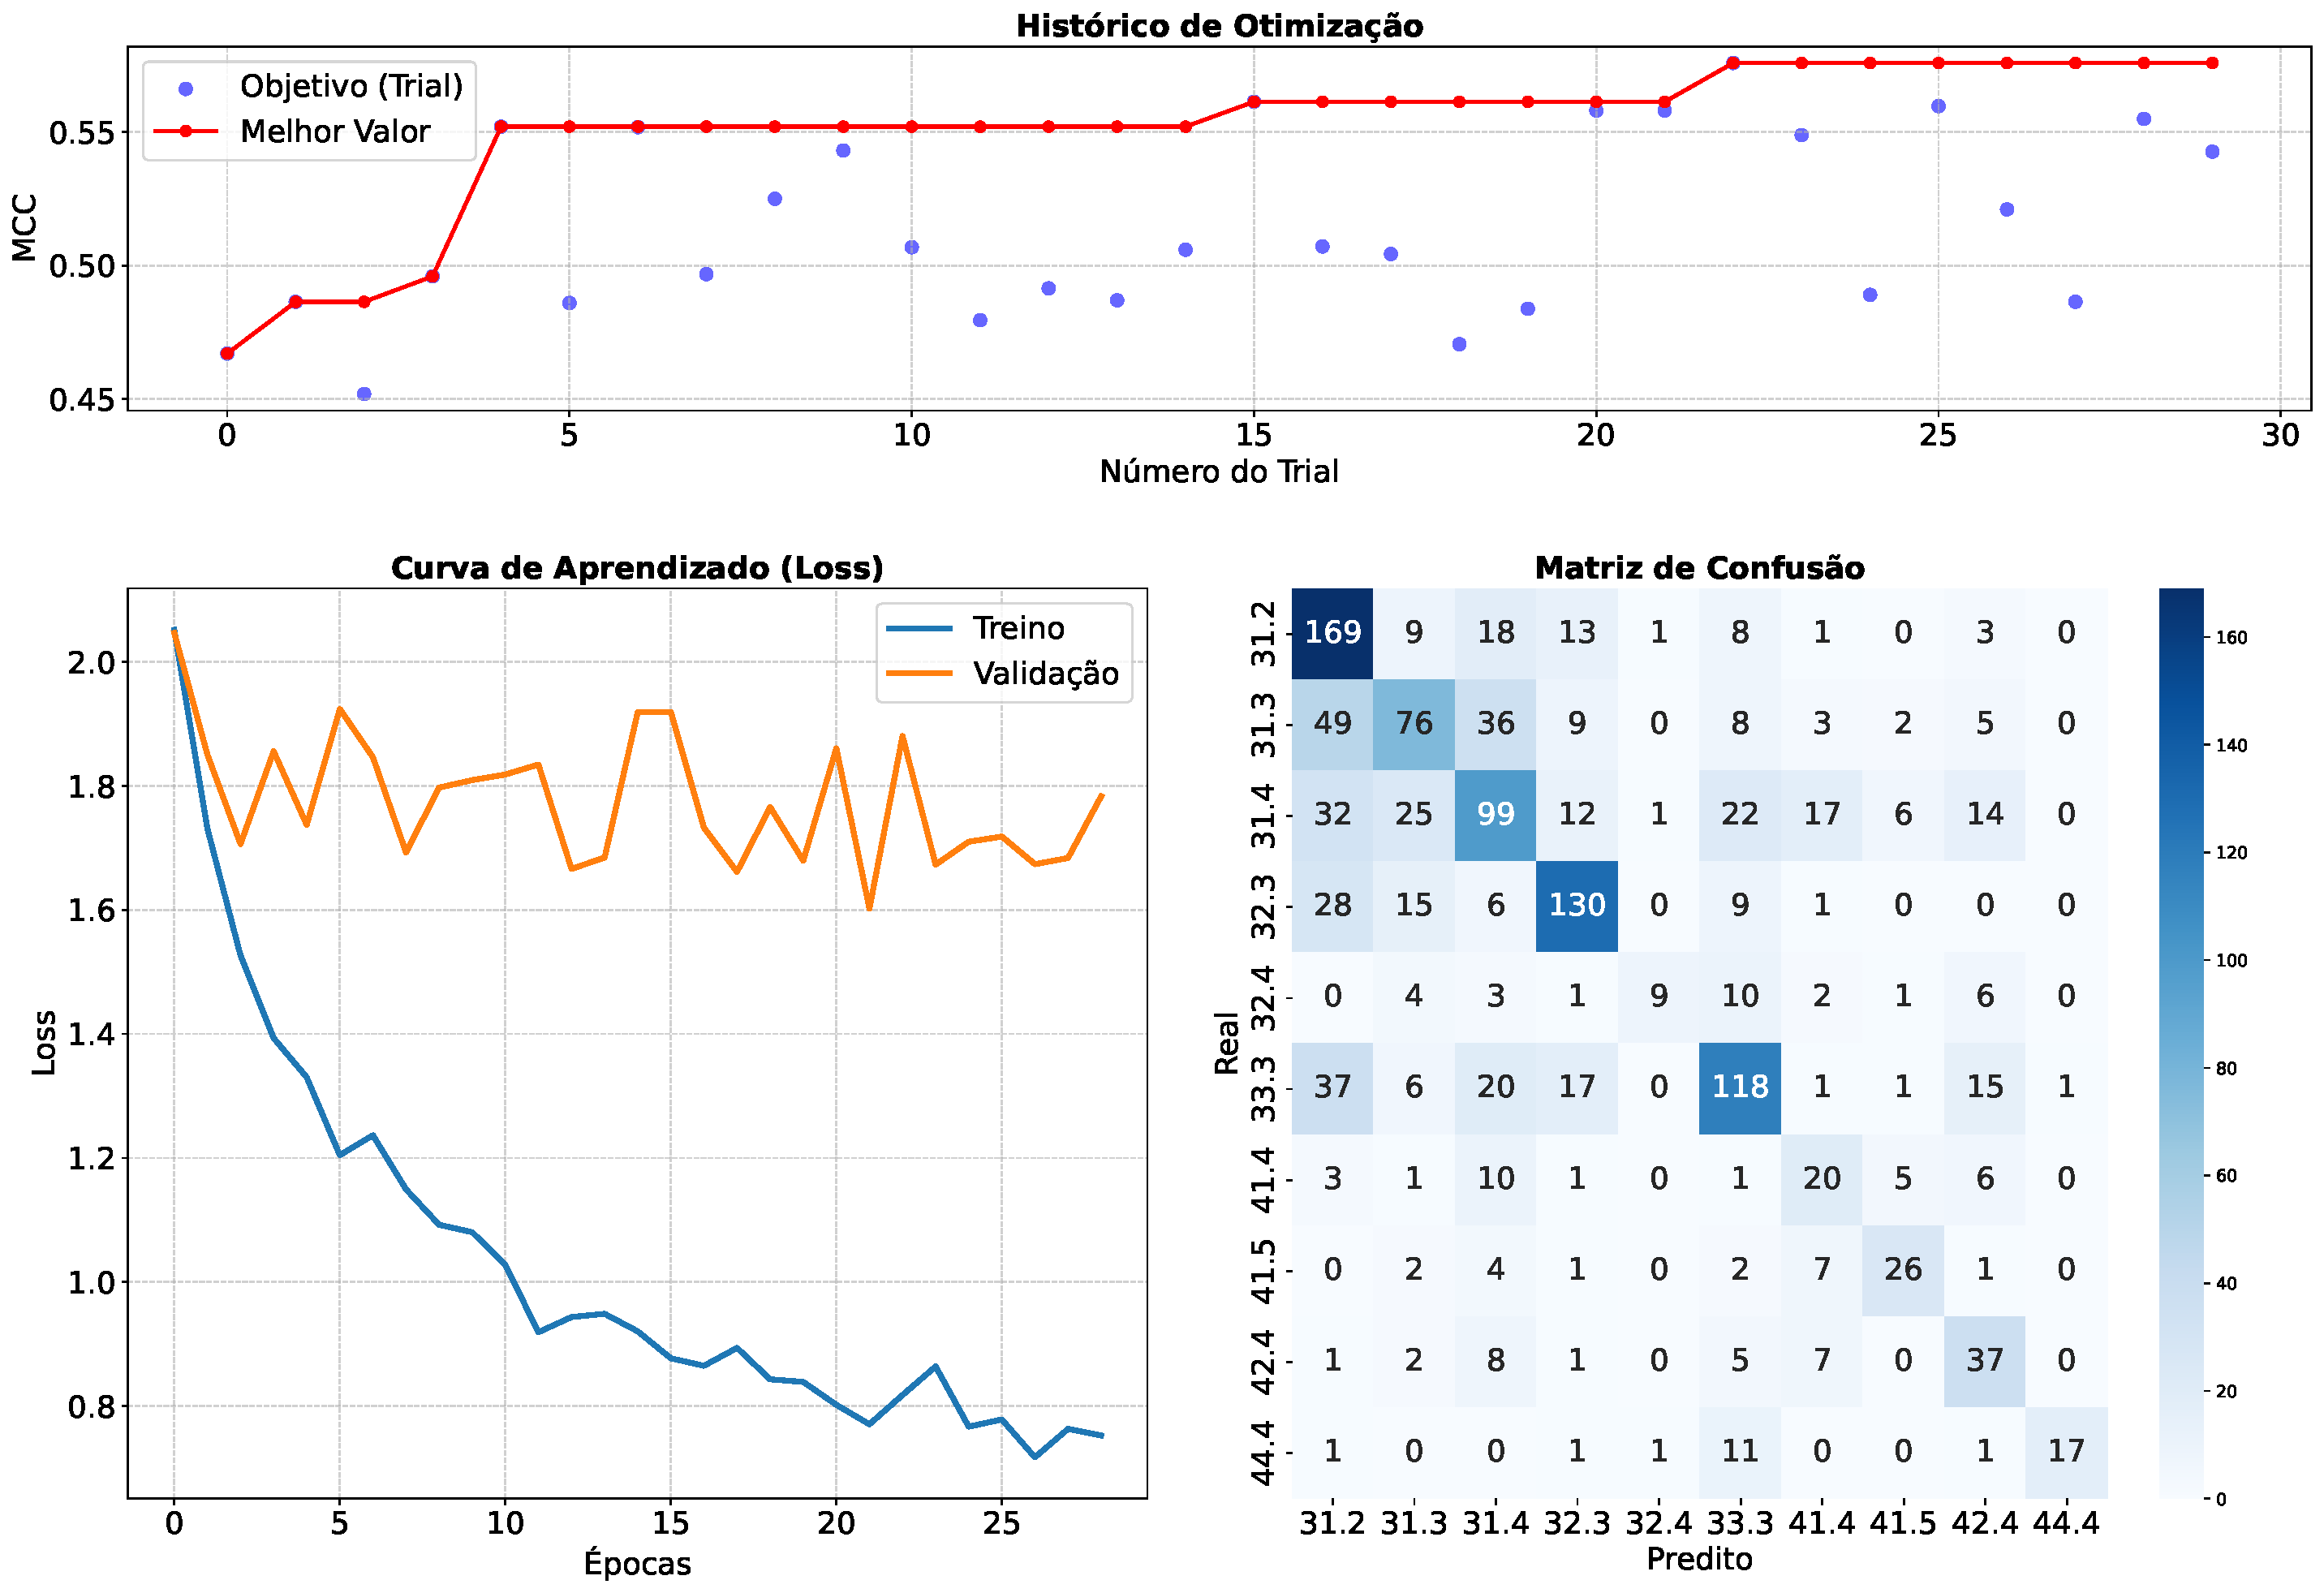
\includegraphics[width=0.85\textwidth]{tex/appendix/experiments/resnet_v10_BR_opt_aug/dashboard_consolidado.pdf}
        \caption{Histórico de Otimização, Curvas de Aprendizado e Matriz de Confusão - resnet\_v10\_BR\_opt\_aug}
    \end{figure}
\end{minipage}
\clearpage
